\documentclass[11pt]{article}
\usepackage{times}
\usepackage{comment} % enables the use of multi-line comments (\ifx \fi)
\usepackage{fullpage} % changes the margin
\usepackage{graphicx}
\usepackage{subcaption}
\usepackage[margin=0.9in]{geometry}

\begin{document}
%Header-Make sure you update this information!!!!
\noindent
\large\textbf{Line W Analysis Update} \hfill \textbf{Jordan Thomas} \\
08/07/2017 \\

\section*{How can age and oxygen become decoupled?}

Age and oxygen are typically expected to be strongly negatively correlated in the
ocean interior (ventilated regions?). Under what conditions does this negative
relationship break down, and even reverse?


\section*{Results - Model Age-Oxygen Relationship:}
ESM2Mc model output along Line W suggests a region in the ocean interior where
this relationship is reversed (Figure 1). Scatter analysis of age and oxygen
in this region (distance averaged between 600--900 km) indicates that this positive correlation
area occurs when there is a larger gradient in age than oxygen (Figure 2). This
suggests that the positive correlation could be due isopycnal heave.

\begin{figure*}[b!]
    \centering
    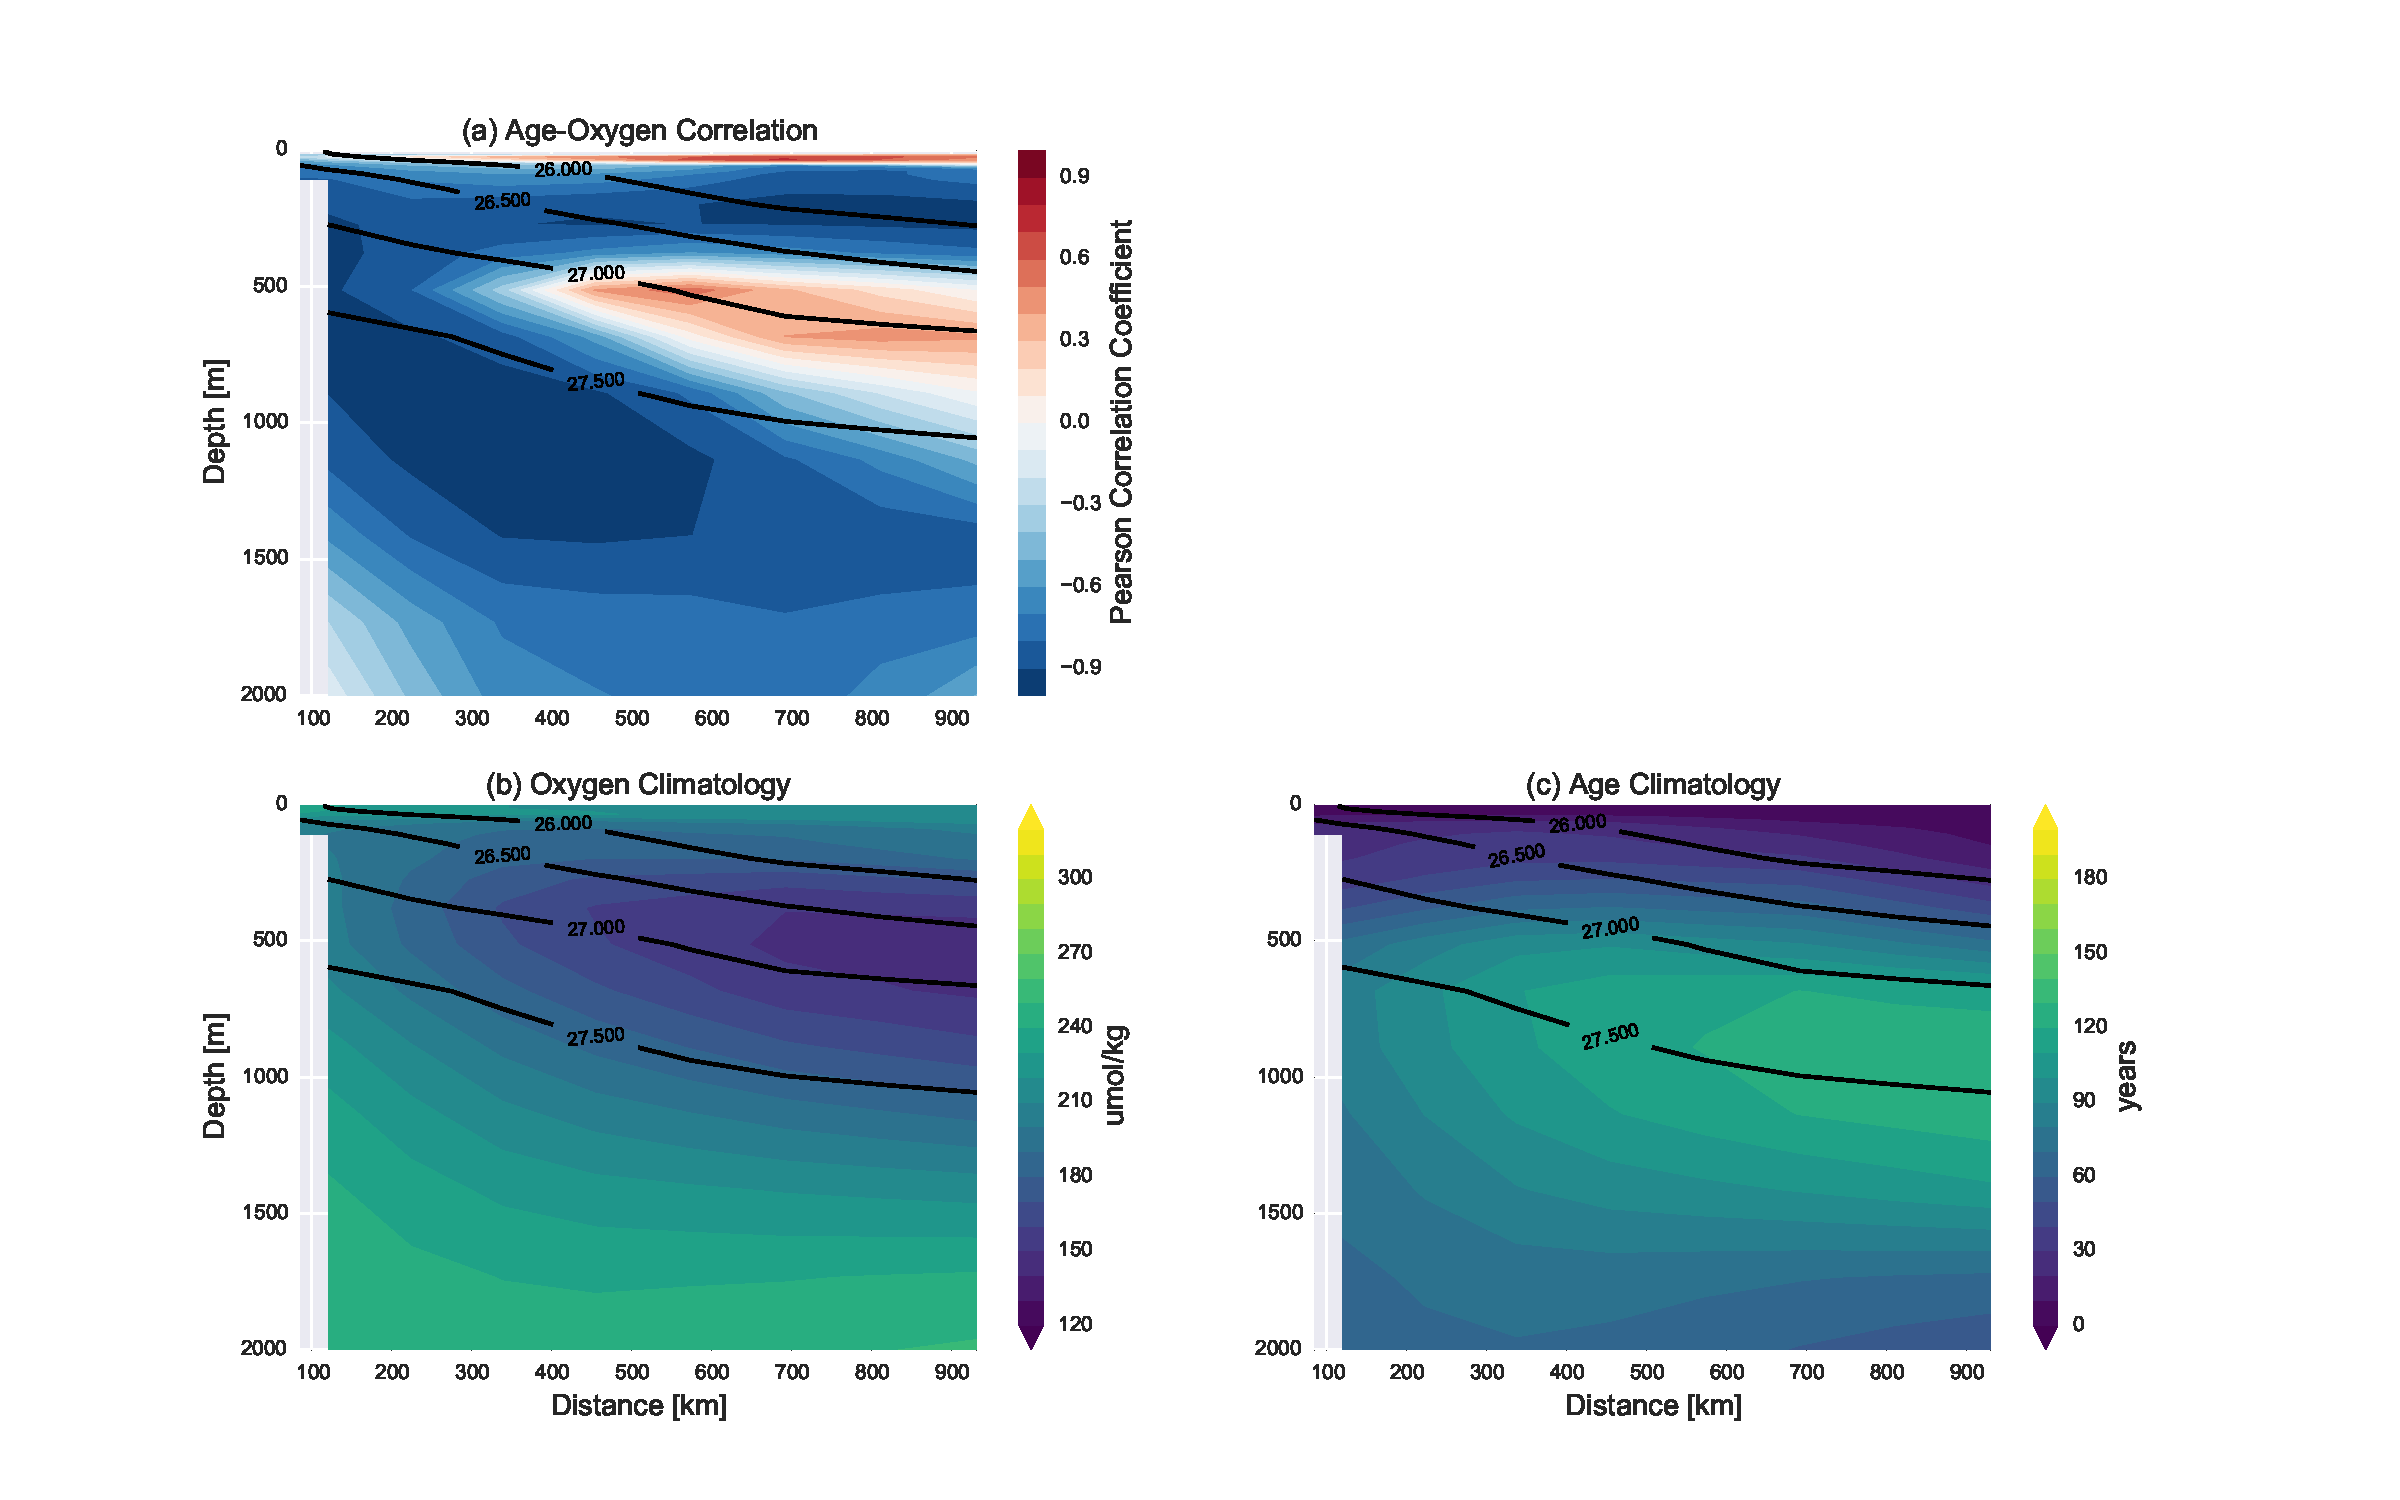
\includegraphics[height=5in]{correlation_clim_on_linew.pdf}
    \caption{(a) Pearson correlation coefficient for age vs oxygen interpolated to
    Line W. (b) oxygen climatology and (c) age climatology on Line W.}
\end{figure*}

\begin{figure*}[t!]
    \centering
    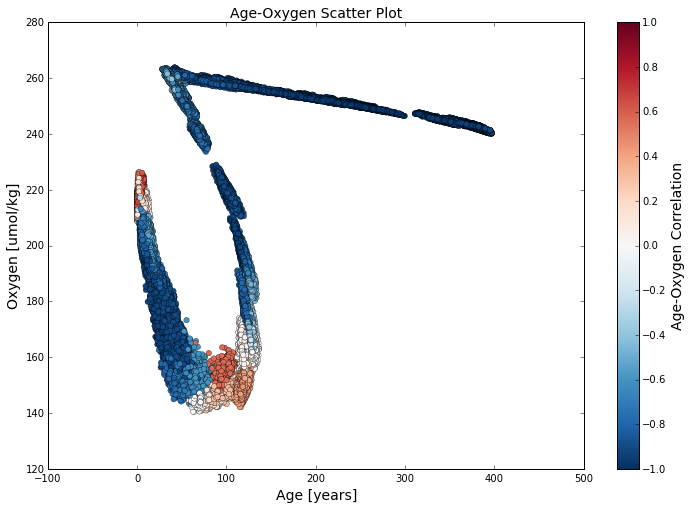
\includegraphics[height=3.7in]{Age-Oxygen_scatter.png}
    \caption{Scatter plot of age and oxygen averaged between distances 600--900
    km. Colors indicate correlation coefficient.}
\end{figure*}

To explore why there is a positive correlation in this region at this depth, we
partition the correlation between age and oxygen into two terms: the correlation
on a constant density surface ($\gamma_n = 27.0$) and the correlation due to the
vertical displacement of the density surface (heave). These two terms are referred to
as `no heave' and `pure heave' respectively.

To calculate these two terms first the correlation between age and oxygen is calculated
on the average depth of the $\gamma_n = 27.0$ density surface:

\begin{equation}
r_{\mathrm{total}} = corr(\mathrm{age},\: \mathrm{o_2})\bigg\vert_{\overline{\gamma_n}=27.0}
\end{equation}

Next the no heave term is calculated by taking the correlation of age and oxygen
interpolated to the $\gamma_n = 27.0$ surface at each time-step.

\begin{equation}
r_{\mathrm{no\ heave}} = corr(\mathrm{age}|_{\gamma_n = 27.0},\: \mathrm{o_2}|_{\gamma_n = 27.0})
\end{equation}

Finally the pure heave term is calculated as the difference between the total
correlation and the no heave correlation.

\begin{equation}
r_{\mathrm{pure\ heave}} = r_{\mathrm{total}} - r_{\mathrm{no\ heave}}
\end{equation}

Figure 3 shows that the positive correlation region at the end of Line W is entirely
do to the localized vertical displacement of the isopycnal surfaces.

\begin{figure*}[t!]
    \centering
    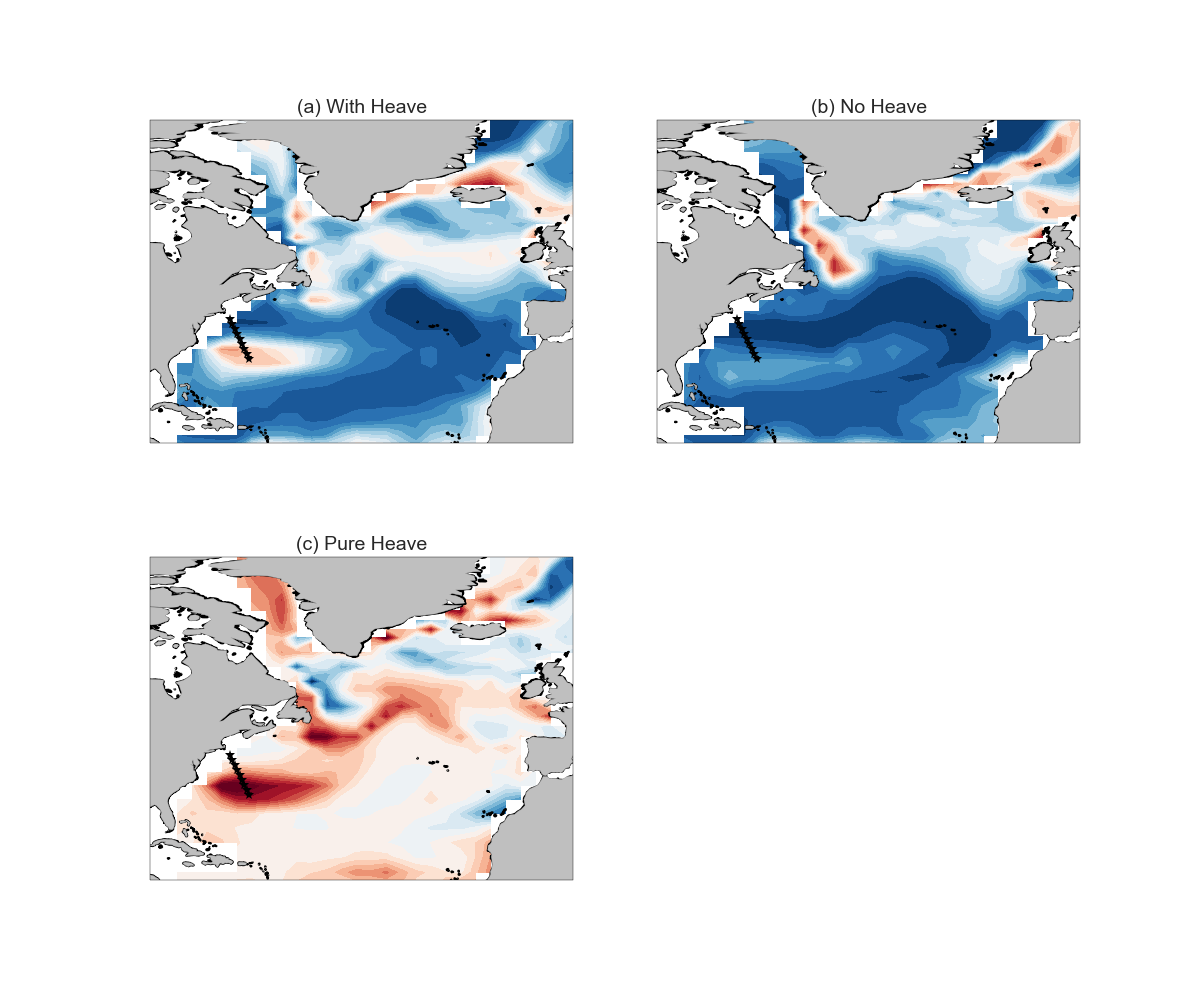
\includegraphics[height=6in]{correlation_heave.png}
    \caption{Correlation coefficient between age and oxygen on neutral density
    $\gamma_n = 27.0$. (a) shows the correlation on the average depth of the
    isopycnal, (b) shows the correlation with the effects of isopycnal heave removed,
    and (c) shows the difference between these two, i.e. the impact of isopycnal
    heave on the correlation.
    }
\end{figure*}


\clearpage


\end{document}
